\section{方法}

\subsection{总体流程}
本文方法的总体流程如图~\ref{fig:framework} 所示。输入 RGB 低照度图像后，首先转换到 YCbCr 空间，仅在亮度通道 $Y$ 上进行增强；随后在平滑亮度图上计算 tile 级结构方差，并利用残差域噪声估计执行噪声扣除；接着通过分位数归一化和幂函数映射生成 clip map；最后对每个 tile 构建局部 CLAHE-LUT，并在相邻 tile 之间进行双线性插值融合，得到增强亮度图，再与色度通道重组为输出图像。

\begin{figure}[H]
\centering
\refstepcounter{figure}\label{fig:framework}
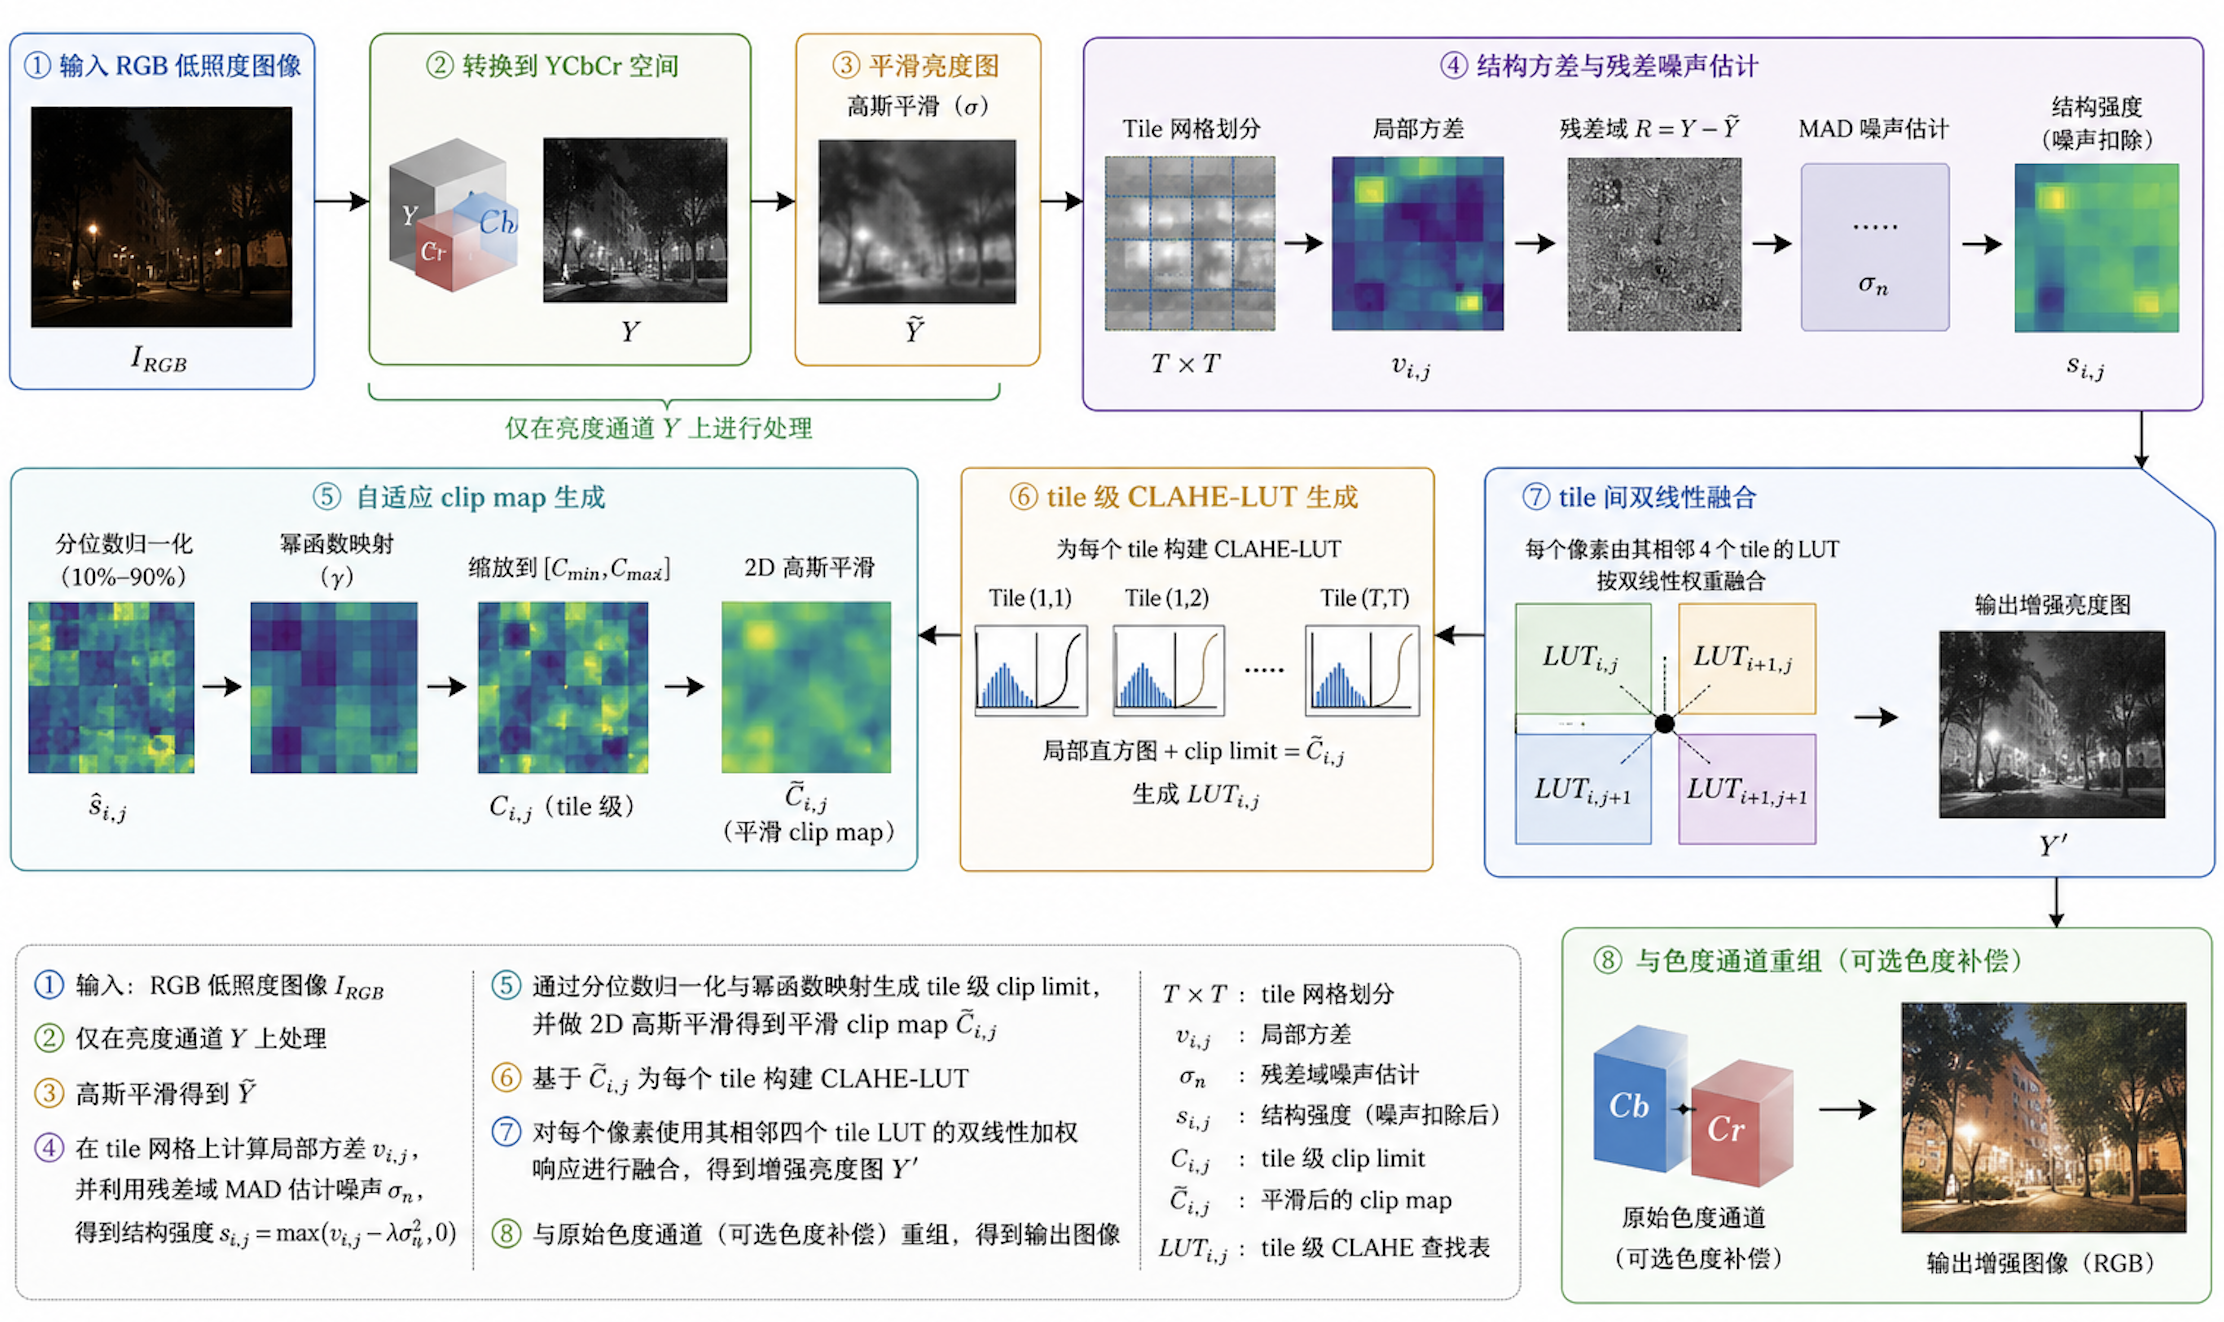
\includegraphics[width=\linewidth]{../figures/figure1_overall_pipeline_body.png}
\end{figure}

\subsection{噪声抑制结构方差}
设输入亮度图为 $Y$，先进行高斯平滑得到
\begin{equation}
\tilde{Y}=G_{\sigma}*Y.
\end{equation}
然后在 tile 网格上计算局部方差
\begin{equation}
v_{i,j}=\mathrm{Var}(\tilde{Y}_{i,j}).
\end{equation}

首轮实验表明，若直接用 Laplacian 高频响应估计噪声并从亮度方差中扣除，会出现量纲不一致的问题。为此，本文采用残差域
\begin{equation}
R = Y-\tilde{Y}
\end{equation}
上的 MAD（Median Absolute Deviation）估计噪声标准差：
\begin{equation}
\sigma_n = \frac{\mathrm{median}(|R-\mathrm{median}(R)|)}{0.6745}.
\end{equation}
相应地，tile 级结构强度定义为
\begin{equation}
s_{i,j} = \max(v_{i,j}-\lambda \sigma_n^2,0),
\end{equation}
其中 $\lambda$ 为噪声扣除强度系数。

\subsection{自适应 clip map 生成}
直接将 $s_{i,j}$ 代入有理函数映射时，容易出现 clip limit 动态范围过窄的问题。针对这一问题，本文先对结构强度图进行分位数归一化：
\begin{equation}
\hat{s}_{i,j} = \mathrm{clip}\left(\frac{s_{i,j}-P_{10}(s)}{P_{90}(s)-P_{10}(s)+\epsilon}, 0, 1\right),
\end{equation}
其中 $P_{10}(s)$ 和 $P_{90}(s)$ 分别表示结构强度的 10\% 和 90\% 分位数。随后利用幂函数生成 tile 级 clip map：
\begin{equation}
C_{i,j}=C_{\min}+(C_{\max}-C_{\min})\hat{s}_{i,j}^{\gamma}.
\end{equation}
其中 $\gamma$ 与参数 $\beta$ 关联，用于控制高结构区域的增强幅度。最后对 tile 级参数图做一次二维高斯平滑，以减小相邻 tile 之间的参数突变。

\subsection{tile 级映射与双线性融合}
对于每个 tile，本文构建一个对应的 CLAHE-LUT。首轮实现中采用“逐 tile 硬拼接”方式，导致不同 tile 间边界突变明显。为此，本文进一步将每个像素的输出值表示为其相邻四个 tile LUT 响应的双线性组合：
\begin{equation}
Y'(x,y)=\sum_{m,n} w_{m,n}(x,y)\,T_{m,n}(Y(x,y)),
\end{equation}
其中 $T_{m,n}$ 表示第 $(m,n)$ 个 tile 的 LUT 映射，$w_{m,n}$ 为满足归一化条件的双线性插值权重。该设计使 tile 间过渡更加平滑，从而减弱块状伪影。

\subsection{可选色度补偿}
实验发现，若在合成数据定量实验中直接施加较强色度补偿，会明显影响 RGB 统计分布并拉低 RGB-SSIM。因此本文将色度补偿从核心定量增强流程中剥离，仅在真实低照度视觉展示时采用轻量色度补偿：
\begin{equation}
g(x)=\left(\frac{Y'(x)+\epsilon}{Y(x)+\epsilon}\right)^{\delta},
\end{equation}
\begin{equation}
C_r'(x)=128+\eta g(x)(C_r(x)-128),\quad
C_b'(x)=128+\eta g(x)(C_b(x)-128).
\end{equation}
其中 $\eta$ 为补偿强度系数，$\delta$ 为增益压缩系数。
